
\begin{itemize}
\item 
The document should display your full name and student number. 
\item 
The file should be a pdf whose name contains your family name
\item 
Layout: is the document visually pleasing? Is it well structured? 
\item Is there a complete bibliography (when applicable)?
\item Does the structure follows this: Introduction - Methods - Results - Discussion - Conclusion - Appendix ?
\item 
Figures: Are they properly numbered? captioned? all figures must be referenced in the text. Are they of good quality? are they readable? are all axis labelled?
\item 
Text: Overall quality of the language. Are there still typos? Do all sentence make sense? 
\item 
Discussion: are the results properly discussed, analyzed? are potential problems, errors, limitations discussed?
\item 
Conclusion: Are the report's findings summarized and generalized?
\end{itemize}

\begin{center}
\begin{tabular}{cc}
\hline
No & Yes \\
\hline
\hline
$6.67*10^{-11}$ & $6.67 \times 10^{-11}$ \\
$kg/m^3$ Yes: kg/m$^{3}$ or kg.m$^{-3}$\\
1x1 & 1$\times$1\\
$cos$ & $\cos$\\
docx file & pdf file \\
'if you do this'& passive form \\ 
\hline
\end{tabular}
\end{center}




%.....................................
\par\noindent\rule{\textwidth}{0.4pt}
\begin{center}
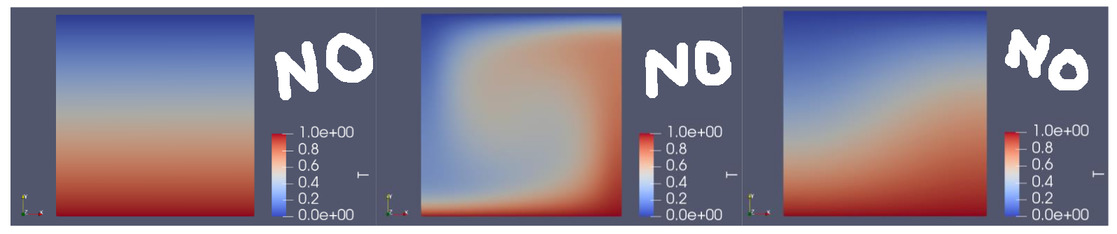
\includegraphics[width=10cm]{images/grading/grey}\\
No grey background
\end{center}


%.....................................
\par\noindent\rule{\textwidth}{0.4pt}
\begin{center}
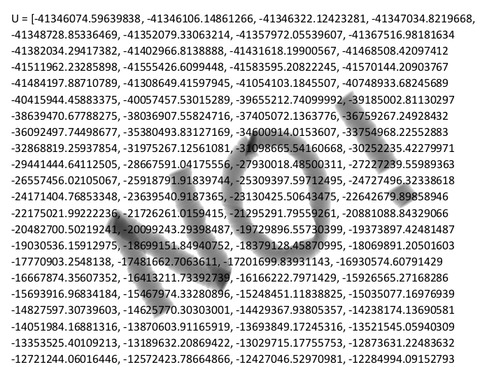
\includegraphics[width=8cm]{images/grading/numbers}\\
No lists/arrays with numbers
\end{center}

%.....................................
\par\noindent\rule{\textwidth}{0.4pt}
\begin{center}
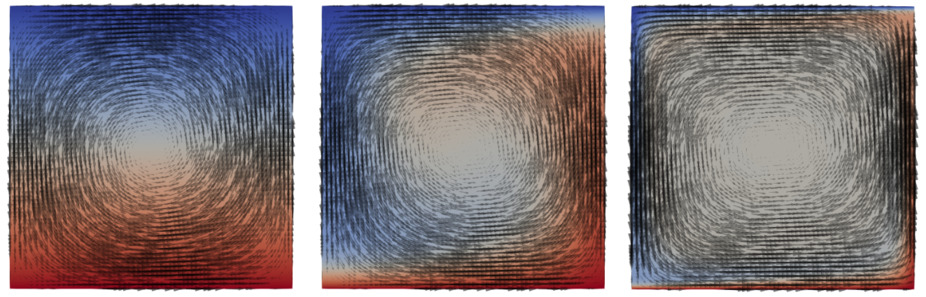
\includegraphics[width=10cm]{images/grading/arrows2}\\
Too many arrows\\
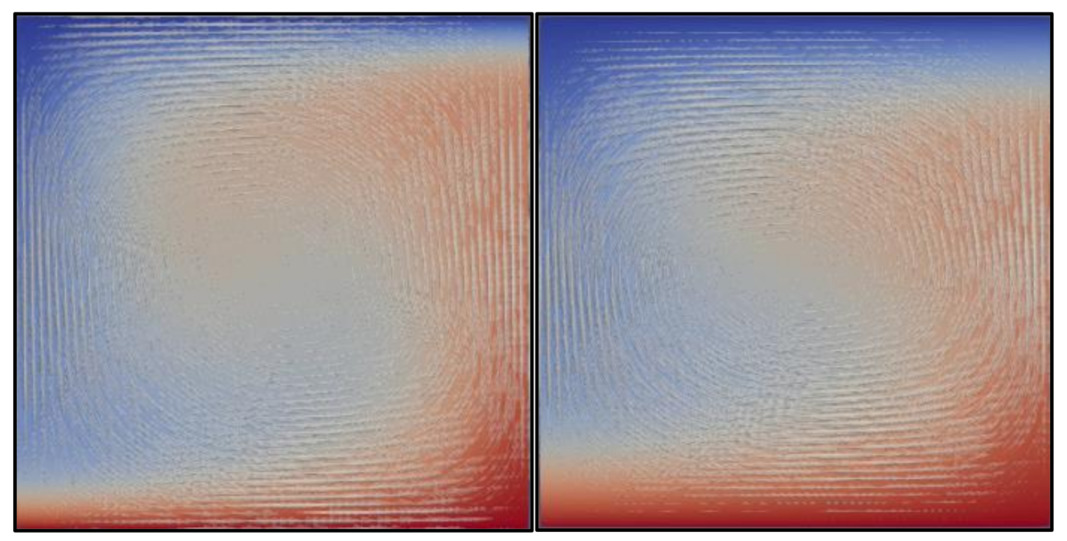
\includegraphics[width=9cm]{images/grading/arrows1}\\
Poor choice of arrow colour
\end{center}

%.....................................
\par\noindent\rule{\textwidth}{0.4pt}
\begin{center}
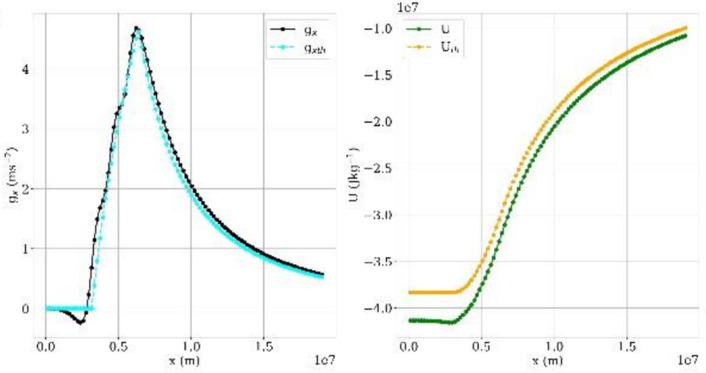
\includegraphics[width=8cm]{images/grading/pixels1}
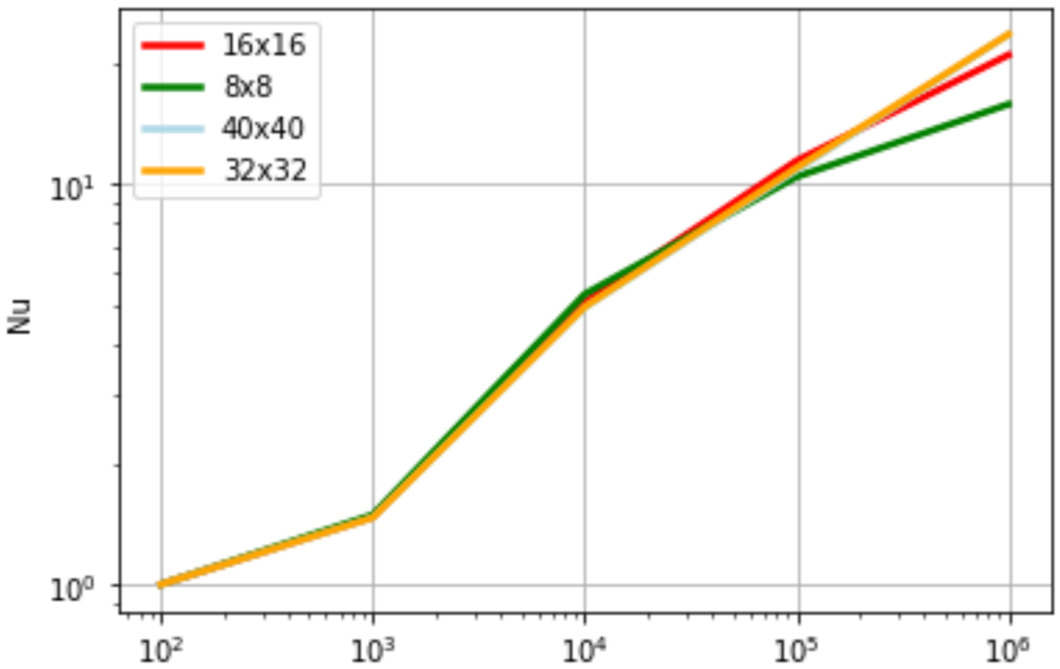
\includegraphics[width=7cm]{images/grading/pixels2}\\
Be careful about how you export your figures. These are unreadable.
\end{center}
 
%.....................................
\par\noindent\rule{\textwidth}{0.4pt}
\begin{center}
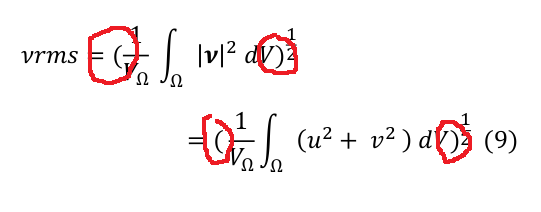
\includegraphics[width=8cm]{images/grading/eqs1}\\
Parenthesis too small
\end{center}

%.....................................
\par\noindent\rule{\textwidth}{0.4pt}
\begin{center}
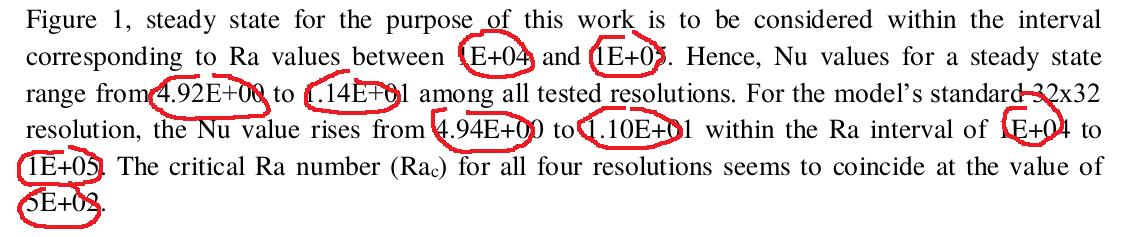
\includegraphics[width=9cm]{images/grading/eqs2}\\
1.6E+10 is not acceptable. Replace by $1.6\cdot 10^{10}$
\end{center}

%.....................................
\par\noindent\rule{\textwidth}{0.4pt}
\begin{center}
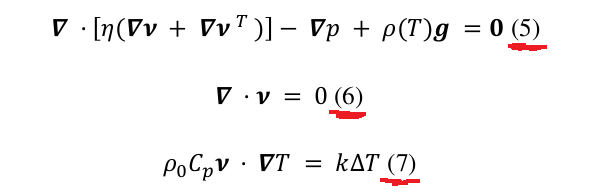
\includegraphics[width=7cm]{images/grading/eqs3}\\
Equation number is too close to the equation itself.
\end{center}

%.....................................
\par\noindent\rule{\textwidth}{0.4pt}
\begin{center}
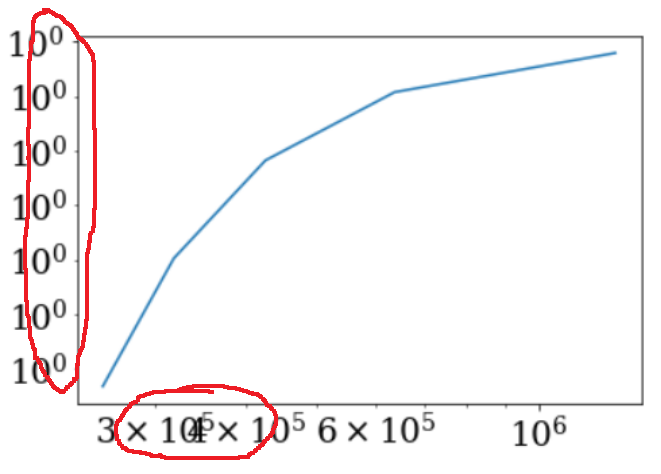
\includegraphics[width=9cm]{images/grading/eqs4}\\
Formatting of both axis lead to unreadable figure.
\end{center}

%.....................................
\par\noindent\rule{\textwidth}{0.4pt}
\begin{center}
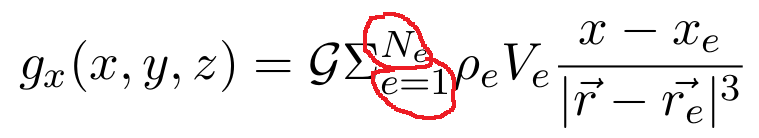
\includegraphics[width=9cm]{images/grading/eqs5}\\
In \LaTeX{}  use \verb!\sum\limits!
\end{center}

%.....................................
\par\noindent\rule{\textwidth}{0.4pt}
\begin{center}
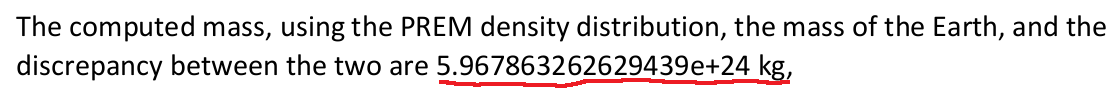
\includegraphics[width=9cm]{images/grading/eqs6}\\
Are so many digits necessary?
\end{center}

